\documentclass[a4paper,12pt]{book}
\usepackage[utf8]{inputenx} 
\usepackage[spanish]{babel} 
\usepackage[left=2cm,right=2cm,top=2cm,bottom=2cm]{geometry}
\usepackage{scrextend}
\usepackage{marvosym}
\usepackage{pifont} % Generación de símbolos especiales
\usepackage{textcomp}
\usepackage{newpxtext}
\usepackage{newpxmath}
\usepackage[T1]{fontenc} % Codificación de salida    
\usepackage{microtype} % Mejoras det microtipografía en la obtención de PDF (sólo para pdflatex)
\usepackage[hyphens]{url} % Para escritura de URL
\urlstyle{sf} % Estilo de URL sin serifas para que tengan un mejor aspecto
\usepackage{tikz}
% Paquetes para obtener un mayor control de las listas
\usepackage{paralist} % Mayor control de listas
\usepackage{multicol} % Elementos en varias columnas

\usepackage[pdftex]{hyperref}
\hypersetup{colorlinks=true,linkcolor=black} 
\usepackage{graphicx}
\usepackage{listings}
\usepackage{caption}
\captionsetup[figure]{labelformat=empty}

\usepackage{color}
\definecolor{gray97}{gray}{.97}
\definecolor{gray75}{gray}{.75}
\definecolor{gray45}{gray}{.45}
\lstset{ frame=Ltb,
	framerule=0pt,
	aboveskip=0.5cm,
	framextopmargin=3pt,
	framexbottommargin=3pt,
	framexleftmargin=0.4cm,
	framesep=0pt,
	rulesep=.4pt,
	backgroundcolor=\color{gray97},
	rulesepcolor=\color{black},
	%
	stringstyle=\ttfamily,
	showstringspaces = false,
	basicstyle=\small\ttfamily,
	commentstyle=\color{gray45},
	keywordstyle=\bfseries,
	%
	numbers=left,
	numbersep=15pt,
	numberstyle=\tiny,
	numberfirstline = false,
	breaklines=true,
}

% minimizar fragmentado de listados
\lstnewenvironment{listing}[1][]
{\lstset{#1}\pagebreak[0]}{\pagebreak[0]}

\lstdefinestyle{consola}
{basicstyle=\scriptsize\bf\ttfamily,
	backgroundcolor=\color{gray75},
}

\lstdefinestyle{Java}
{language=Java,
}
\lstdefinestyle{Python}
{language=Python,
}

\begin{document}

\author{Javier Monescillo Buitrón}
\title{Apuntes de la asignatura Procesadores de Lenguajes}
\date{\today}

\frontmatter
\maketitle
\tableofcontents


\mainmatter
\chapter{Introducción}

\section{Definiciones introductorias}

\begin{itemize}
	\item \textbf{Procesador}: Sistema cuyo objetivo es el procesamiento de una entrada con el fin de producir una salida.
	\item \textbf{Lenguaje}: Conjunto de cadenas formadas por elementos tomados de un alfabeto.
	\item \textbf{Procesador de lenguajes}: Toma como entrada cadenas de un lenguaje, que son procesadas para producir una salida.
	\item \textbf{Traductor}: Entrada texto en $L_1$ (lenguaje fuente) y salida texto en $L_2$ (lenguaje objeto, preservando el significado).
	\item \textbf{Intérprete}: procesa las instrucciones del lenguaje fuente y las ejecuta, NO las traduce.
\end{itemize}

\begin{figure}[h]
	\centering
	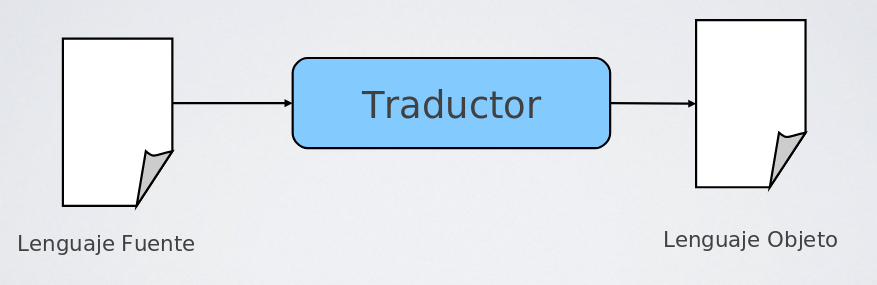
\includegraphics[width=0.7\linewidth]{img/1}
	\caption{}
	\label{fig:1}
\end{figure}

\textbf{Tipos de traductores:}
\begin{center}
	\begin{tabular}{|c|c|c|}
		\hline 
		& \textbf{Lenguaje fuente (L1)} & \textbf{Lenguaje objeto (L2)}  \\ 
		\hline 
		Compilador & Lenguaje alto nivel & Lenguaje máquina  \\ 
		\hline 
		Ensamblador & Lenguaje ensamblador & Lenguaje máquina  \\ 
		\hline 
		Preprocesador & L. Alto nivel con extensiones & L. Alto Nivel sin extensiones \\ 
		\hline 
		Conversor fuente-fuente & Lenguaje de Alto nivel & Lenguaje de Alto nivel (distinto)  \\ 
		\hline 
		Decompilador & Lenguaje de Bajo nivel & lenguaje de Alto nivel \\ 
		\hline 
	\end{tabular} 
\end{center}

\section{Lenguajes, gramáticas y autómatas}
\textbf{¿Qué es una gramática?}\newline
Las gramáticas son un ente formal para especificar de manera finita, el conjunto de cadena de símbolos potencialmente infinitos que constituyen un lenguaje.
Una gramática es una cuádrupla(V,T,P,S):
\begin{itemize}
	\item V: símbolos no terminales.
	\item T: símbolos terminales.
	\item P: reglas de producción.
	\item S: símbolo inicial de la gramática.
\end{itemize}
Podemos definir las cadenas que pertenecen al lenguaje por \textbf{extensión} o por \textbf{derivación} (a partir de su gramática y símbolo inicial). Existen varios tipos de gramáticas:
\begin{itemize}
	\item \textbf{Gramática tipo 0}: Sin restricciones o de estructuras de frases.
	\item \textbf{Gramática tipo 1}: Sensibles al contexto.
	\item \textbf{Gramática tipo 2}: Independientes del contexto.
	\item \textbf{Gramática tipo 3}: Regulares.
\end{itemize}
\begin{figure}[h]
	\centering
	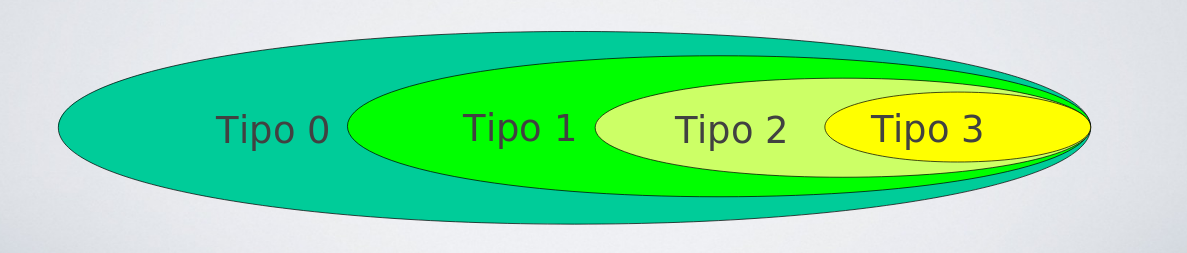
\includegraphics[width=0.5\linewidth]{img/2}
	\caption{}
	\label{fig:2}
\end{figure}

El lenguaje generado por una gramática G=(V,T,P,S), será notado como L(G), y se define como el conjunto de cadenas formadas por símbolos terminales que son derivables a partir del símbolo inicial de la gramática.

\begin{center}
	$L(G)=\{u\epsilon T | S \Rightarrow u\}$
\end{center}

\begin{center}
	\begin{tabular}{|c|c|c|}
		\hline 
		Gramáticas	& Lenguajes  & Máquinas \\ 
		\hline 
		GLC & Libre de contexto & Autómatas a Pila \\ 
		\hline 
		GR & Regular & Autómatas Finitos\\ 
		\hline 
	\end{tabular} 
\end{center}

\section{Derivación de una gramática}
Dada una gramática G(V,T,P,S) y dos palabras $\alpha$,$\beta \epsilon$ (V$\cup$T)$\ast$, solo decimos que $\beta$ es derivable a partir de $\alpha$ en un paso ($\alpha \Rightarrow \beta$) si y solo si existen palabras $\delta_1, \delta_2 \epsilon$ (V$\cup$T)$\ast$ y una producción Y $\longrightarrow \emptyset$ tales que $\alpha = \delta_1$ y $\delta_2$ y $\beta$= $\delta_1 \emptyset \delta_2$
\section{Definición de un lenguaje}
La definición de un lenguaje implica:
\newline
\newline
\textbf{Léxico}: vocabulario del lenguaje junto con sus categorías. Por ejemplo, en un lenguaje de programación, dentro de la categoría tipos, podríamos encontrar el vocabulario (int, float,double, etc).
\newline
\newline
\textbf{Sintáctico}: Reglas que establecen como construir frases válidas del lenguaje usando los elementos del vocabulario.
\newline
\newline
\textbf{Semántico}: El significado de las frases, es la información de la cadena, por ejemplo al leer la cadena, "int v = 0", el significado es "una variable numérica v se asigna el valor 0".
\newline
\newline
El léxico corresponde a un lenguaje regular, por lo que se expresa con una GR. Por otro lado, el sintáctico se corresponde con una GLC (aunque no tiene por qué ser al completo).
\newline
\newline
Para distinguir una GR de un GLC hay que fijarse en la parte derecha de la producción y ver si tiene uno o mas no terminales.

\section{Estructura de un traductor}
El proceso de la traducción implica dos fases:
\begin{itemize}
	\item \textbf{Fase de Análisis}(front end): Comprueba que el texto de entrada esta escrito conforme a las reglas (léxicas y sintácticas del lenguaje). Esta fase es dependiente del lenguaje.
	\item \textbf{Fase de Síntesis} (back end): Genera texto equivalente optimizado en el lenguaje objeto. Esta fase es dependiente de la máquina.
\end{itemize}

\begin{figure}[h]
	\centering
	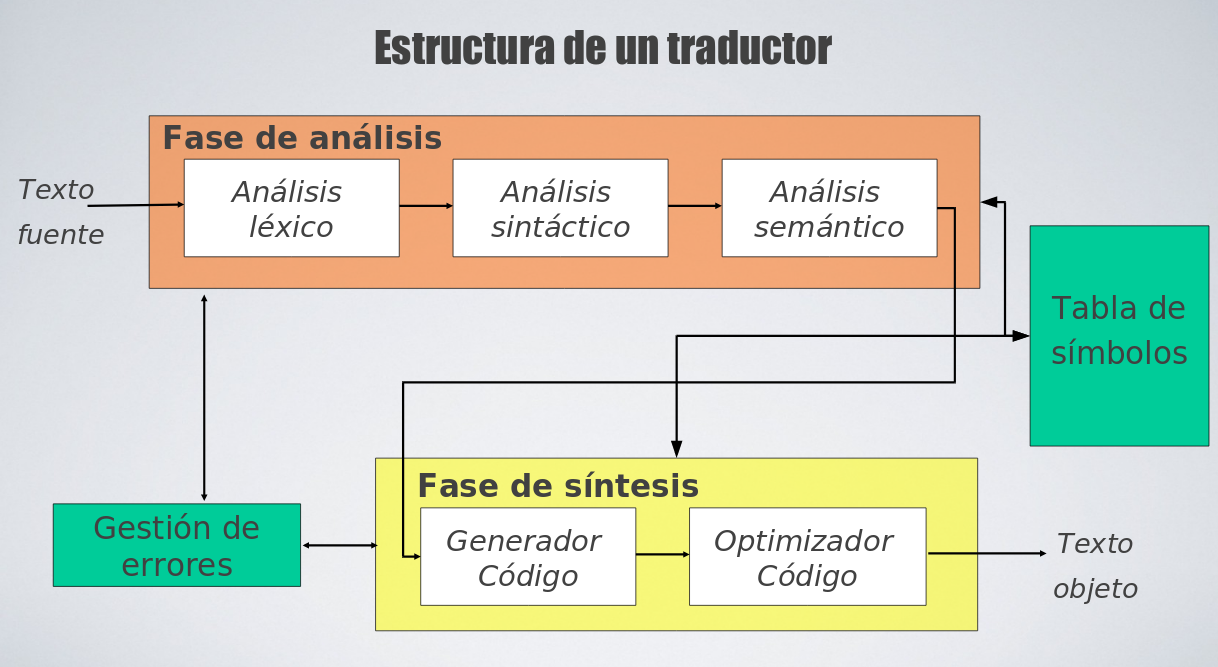
\includegraphics[width=0.7\linewidth]{img/4}
	\caption{}
	\label{fig:4}
\end{figure}

En el análisis léxico se va iterando carácter a carácter, reconociendo si son palabras válidas del lenguaje. Es decir lee
la palabra “int” y deduce la categoría “tipos”. Elimina e ignora espacios, tabuladores, saltos de línea, etc. Después en
el análisis sintáctico se leen las palabras recibidas (una vez de sabe que pertenecen al lenguaje), y se itera desde el
símbolo inicial de la gramática esa secuencia de palabras, así se comprueba que la estructura es correcta. Finalmente,
en el análisis semántico se recibe “el árbol de derivación” (o un equivalente) y se determina que función hace esa
cadena introducida. Cuando sabe su funcionamiento, lo transmite al generador de código, para que el lenguaje objeto
tenga la misma función.

\section{Técnicas de construcción de traductores con T-Diagramas}
Una notación muy útil para describir programas en general y traductores en particular, son los llamados T-Diagramas.
\begin{figure}[h]
	\centering
	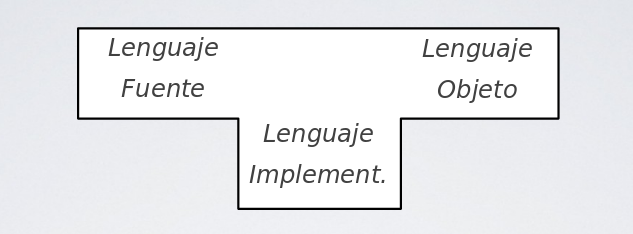
\includegraphics[width=0.7\linewidth]{img/5}
	\caption{}
	\label{fig:5}
\end{figure}


En el siguiente diagrama tipo T se explica el funcionamiento del procesador que se pretende implementar, tomamos \textbf{ Mor } como lenguaje fuente, y Java como lenguaje objeto, y además el lenguaje que implementa es Java, es decir, nuestro compilador compila a Java, y esta escrito a Java. 
\newline
\newline
Para utilizar ese compilador, utilizamos un compilador auxiliar, que está escrito en código máquina para dar lugar a bytecode, el típico archivo \textbf{.class} que generamos al compilar un \textbf{.java}.
\newline

Por último tenemos que compilar el bytecode, con un compilador que acepta bytecode escrito en código máquina.
\begin{figure}[h]
	\centering
	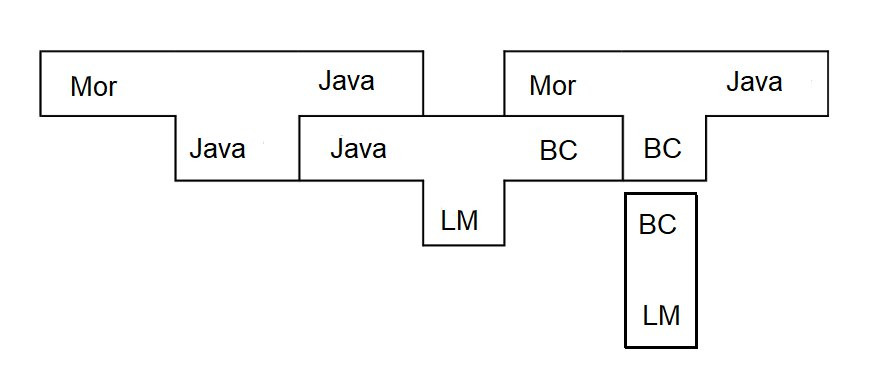
\includegraphics[width=0.7\linewidth]{img/photo5978652419892031524}
	\caption{}
	\label{fig:photo5978652419892031524}
\end{figure}




\chapter{Análisis léxico}
\section{¿Cuando interesa utilizar un Procesador de Lenguajes?}
Cuando quiero hacer la comunicación en un sistema y dicha comunicación es compleja, hay ocasiones donde me interesa definir un lenguaje con un dominio físico.

\section{¿Cuál es la función del analizador léxico?}
Es función del analizador léxico: 
\begin{itemize}
	\item Reconocer los símbolos o tokens que componen el texto fuente.
	\item Eliminar comentarios del texto fuente.
	\item Eliminar los espacios en blanco, saltos de línea y página, tabuladores
	\item Avisar de los errores léxicos detectados.
\end{itemize}

\begin{figure}[h]
	\centering
	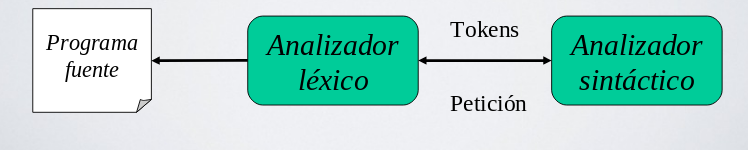
\includegraphics[width=0.7\linewidth]{img/lex1}
	\caption{}
	\label{fig:lex1}
\end{figure}

El analizador léxico es el único que interactúa con la entrada, no se detiene al encontrar los primeros errores.
\clearpage
Un ejemplo de funcionamiento del analizador léxico.
\begin{figure}[h]
	\centering
	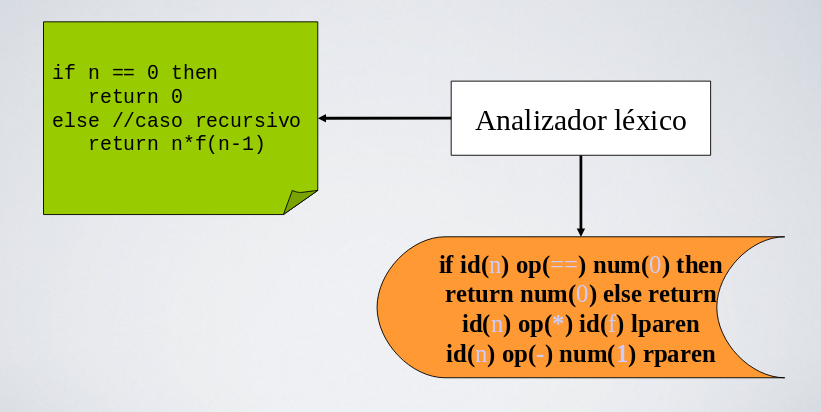
\includegraphics[width=0.7\linewidth]{img/lex2}
	\caption{}
	\label{fig:lex2}
\end{figure}

\section{Función del analizador léxico}
\begin{itemize}
	\item \textbf{Token}: un token es uno o varios elementos básicos del lenguaje fuente que tienen un significado propio. Ejemplos de tokens, presentes en todos los lenguajes de programación, identificadores, palabras reservadas,...
	\item \textbf{Lexema}: es \textit{if} por ejemplo, una combinación concreta de símbolos que forman un token.
	\item \textbf{Patrón}: regla asociada al token que describe a un conjunto de lexemas
\end{itemize}
Son símbolos terminales de la GLC que se van a encargar de comprobar que la estructura del lenguaje es válida, al analizador léxico no le importan los espacios, ni los tabuladores, solo le interesa que la secuencia sea correcta.
\newline
\newline
Es útil estudiar análisis léxico para el reconocimiento de patrones.
\newline
\newline
El problema es encontrar lexemas y disparar patrones, mediante una gramática regular especificamos los lexemas.

	\begin{center}
	\begin{tabular}{|c|c|c|}
		\hline 
		\textbf{Token} & \textbf{Lexema} & \textbf{Patrón} \\ 
		\hline 
		moore & moore & m$\cdot$o$\cdot$o$\cdot$r$\cdot$e  \\ 
		\hline 
		estados &estados & e$\cdot$s$\cdot$t$\cdot$a$\cdot$d$\cdot$o$\cdot$s \\ 
		\hline 
		estado$\_$in & estado$\_$in & e$\cdot$s$\cdot$t$\cdot$a$\cdot$d$\cdot$o$\cdot$$\_$$\cdot$i$\cdot$n \\ 
		\hline 
		alf$\_$in	& alf$\_$in & a$\cdot$l$\cdot$f$\cdot$$\_$i$\cdot$n \\ 
		\hline 
		alf$\_$out	& alf$\_$out & a$\cdot$l$\cdot$f$\cdot$$\_$o$\cdot$u$\cdot$t \\ 
		\hline 
		transicion	& transicion & t$\cdot$r$\cdot$a$\cdot$n$\cdot$s$\cdot$i$\cdot$c$\cdot$i$\cdot$o$\cdot$n \\ 
		\hline 
		comportamiento	& comportamiento & c$\cdot$o$\cdot$m$\cdot$p$\cdot$o$\cdot$r$\cdot$t$\cdot$a$\cdot$m$\cdot$i$\cdot$e$\cdot$n$\cdot$t$\cdot$o \\ 
		\hline 
		Paréntesis abierto	& ( & ( \\ 
		\hline 
		Paréntesis cerrado	& ) & ) \\ 
		\hline 
		Llave abierta	& $\{$ & $\{$ \\ 
		\hline 
		Llave cerrada	& $\}$ & $\}$ \\ 
		\hline 
		Punto y coma	& ; & ; \\ 
		\hline 
		Coma	& , &  , \\ 
		\hline
		Asterisco barra & $\ast/$  & $\ast$$\cdot/$ \\ 
		\hline 
		Barra asterisco & $/\ast$  &  $/$$\cdot$$\ast$ \\ 
		\hline  
		ID	& hola  & [A-Za-z][A-Zaz0-9$\_$]* \\ 
		\hline 
		CMP	& c1 & c[1-9][0-9]* \\ 
		\hline
		CODIGO	& $\#$codigo aquí $\#$  & $\#$$\cdot$ codigo aquí $\cdot$$\#$\\ 
		\hline
		
		
		
	\end{tabular} 	
\end{center}

\section{Ejemplos con JFlex}

TO-DO

\section{Tratamiento de errores}

TO-DO







\chapter{Análisis sintáctico}
\section{¿Qué es un analizador sintáctico?}
Un analizador \textbf{sintáctico} (o parser) es un programa informático que analiza una cadena de símbolos de acuerdo a las reglas de una gramática formal. El término proviene del latín \textit{pars}, que significa parte (del discurso). Usualmente hace parte de un compilador, en cuyo caso, transforma una entrada en un árbol sintáctico de derivación.
\section{Función del analizador sintáctico}
Las funciones del analizador sintáctico son las siguientes:
\begin{itemize}
	\item Analizar la secuencia de tokens y verificar si son correctos sintácticamente.
	\item Obtener una representación interna del texto fuente.
	\item Avisar de los errores sintácticos detectados.
\end{itemize}
\begin{figure}[h]
	\centering
	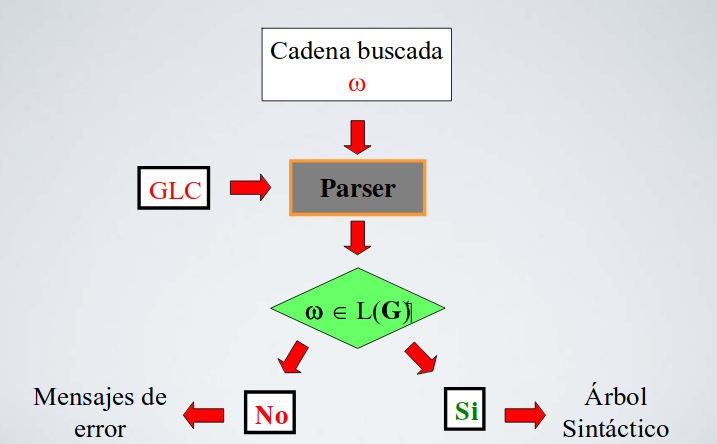
\includegraphics[width=0.7\linewidth]{img/11}
	\caption{Analizador sintáctico}
	\label{fig:5}
\end{figure}
\clearpage
\subsection{Ejemplo funcionamiento}
\begin{figure}[h]
	\centering
	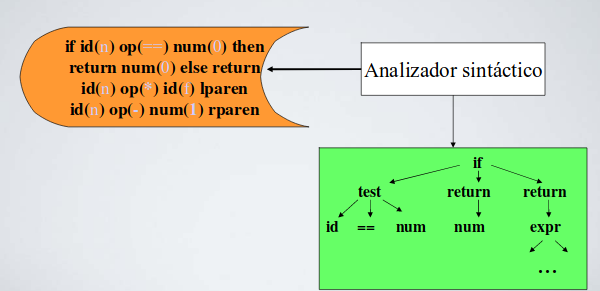
\includegraphics[width=0.7\linewidth]{img/ejemplo_sintactico}
	\caption{}
	\label{fig:ejemplosintactico}
\end{figure}

\textbf{¿Qué necesitamos para poder realizar el análisis sintáctico?}
\newline
Mecanismo para describir las sentencias válidas del lenguaje fuente.
Un sistema que decida ante una entrada ( un programa en texto fuente) si es correcto sintácticamente o no.
\newline
Alguna representación sintáctica del programa.
\newline
\textbf{¿Por qué no se utiliza la misma construcción que en el Analizador Léxico? ¿Por qué no utilizamos AFD's para este tipo de situaciones?}

Porque describir estructuras del tipo $a^nb^n$ usando expresiones regulares es \textbf{imposible}, Lema de Bombeo.
\newline
\newline
\textbf{¿Solución?}

\begin{itemize}
	\item Empleo de construcciones recursivas
	\item Empleo de Gramáticas Libres de Contexto o GLC
\end{itemize}


\section{Gramáticas libres de contexto}

Una gramática libre de contexto se define como la cuádrupla	$G =(V,T,P,S)$
	\begin{itemize}
		\item V: símbolos no terminales de la gramática.
		\item T: símbolos terminales de la gramática.
		\item P, producciones de la gramática.
		\item S, símbolo inicial de la gramática.
	\end{itemize}
Sus producciones P, son de la forma:
\newline
\begin{center}
	$A\Rightarrow\alpha$, donde A$\epsilon$V y $\alpha\epsilon$(V$\cup$T)+
\end{center}
Generalmente se permiten producciones nulas:
\begin{center}
	$A\Rightarrow\epsilon$
\end{center}
\section{Derivación}
El proceso de derivación descrito informalmente consiste en :
\begin{itemize}
	\item Comenzar con el símbolo inicial de la gramática, "S", como cadena de entrada.
	\item Seleccionar un símbolo no-terminal N en la cadena y una producción $N\Rightarrow s_1...s_k$ y cambiar la N por $s_1...s_k$ en la cadena.
	\item Repetir el paso 2, hasta que tengamos una cadena \textbf{w} formada únicamente por símbolos terminales, entonces decimos que \textbf{w} es una cadena generada por la gramática.
\end{itemize}
Principalmente hay dos tipos de derivación:
\begin{itemize}
	\item Derivación más a la izquierda
	\item Derivación más a la derecha
\end{itemize}
Si siempre se sustituye en símbolo terminal más a la izquierda tendremos el primer caso, por el contrario, si es sustituido el más a la derecha tendremos el segundo caso.
\section{Árboles sintácticos}
Un \textbf{árbol sintáctico} es una representación gráfica de las derivaciones realizadas hasta obtener una cadena.
\begin{figure}[h]
	\centering
	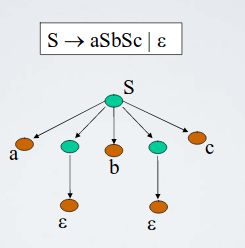
\includegraphics[width=0.5\linewidth]{img/treee}
	\caption{}
	\label{fig:treee}
\end{figure}
\begin{itemize}
	\item Raíz: símbolo inicial de la gramática.
	\item Nodos interiores: símbolos no terminales.
	\item Nodos hojas: símbolos terminales.
\end{itemize}
Cada Nodo interior tendrá como hijos, la parte derecha de la producción aplicada en nodos, ordenados de izquierda a derecha.
\section{Ambigüedad}
Una gramática es \textbf{ambigua} si hay al menos una sentencia que se pueda generar mediante dos o más arboles distintos.
\newline
\newline
Un lenguaje generado por una gramática ambigua es una lenguaje ambiguo.
\newline
\newline
Si todas las gramáticas que generan un determinado lenguaje son ambiguas entonces se dice que el lenguaje es un \textbf{lenguaje inherentemente ambiguo}. 
\newline
\newline 
Nosotros tenemos que trabajar con lenguajes no inherentemente ambiguos.
\newline
\newline
Los analizadores sintácticos deben trabajar con gramáticas no ambiguas.
\section{Estrategias de análisis sintáctico}
\section{Tratamiento de error}
\section{Notacion BNF y EBNF}



\chapter{Análisis sintáctico descendente}
\section{Introducción al análisis sintáctico descendente}

Un \textit{Analizador Sintáctico Descendente} es un tipo de Analizador (ASD) que construye un árbol sintáctico de una Gramática Libre de Contexto (GLC) desde la raíz hasta las hojas. \cite{PL1}
\newline
\newline
Existen dos tipos de Analizadores ASD:
\begin{itemize}
	\item Con retroceso
	\item Sin retroceso
\end{itemize}
Básicamente un \textbf{ASD con retroceso} utiliza un método de fuerza bruta en el que trata de expandir siempre por la primera producción disponible para el símbolo no terminal más a la izquierda. Si son todos los símbolos terminales, entonces finaliza, si no, toca repetir el paso uno hasta finalizar.
\newline
\newline
Este método es muy ineficiente debido a que es probable que no se alcance la cadena del lenguaje a buscar, por lo tanto, habrá muchas vueltas atrás y producciones recursivas a la izquierda que no se pueden parar.
\newline
\newline
La \textbf{recursividad} más a la \textbf{izquierda} es un problema general de cualquier técnica de análisis sintáctico descendente por lo que tenemos que solucionar este problema, se explica más detalladamente en la sección \hyperref[sec:hello]{(5.1)}
\newline
\newline
Sin embargo, los \textbf{ASD sin retroceso} tratan de leer la cadena de izquierda a derecha, predecimos qué producción aplicar en función del símbolo o símbolos actuales de la cadena, así eliminamos las vueltas atrás, por lo que es un Análisis predictivo, tiene la peculiaridad de que solo es aplicable a un tipo especial de gramáticas, denominadas \textbf{LL(1)} y \textbf{LL(k)}.

\clearpage

\section{Gramáticas LL(1) y LL(k)}
Las gramáticas \textbf{LL(k)} son un tipo especial de gramáticas que permiten un análisis descendente sin retroceso. \cite{PL2}
\begin{itemize}
	\item L: leen la cadena de izquierda a derecha \textit{(Left to right)}
	\item L: para generar la cadena utilizan derivaciones más a la izquierda \textit{(Leftmost derivations)}
	\item k. utilizan los \textit{k} primeros símbolos de la cadena para determinar cual es la producción que se debe de aplicar.
\end{itemize}
\begin{figure}[h]
	\centering
	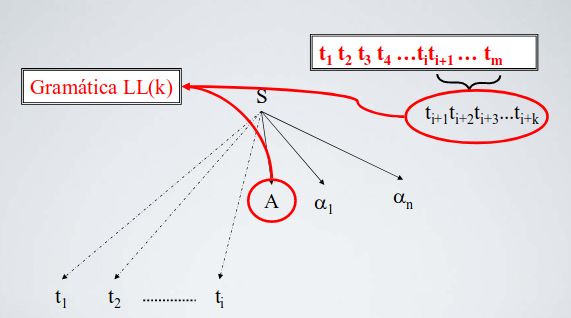
\includegraphics[width=0.5\linewidth]{img/22}
	\caption{Gramática LL(k)}
	\label{fig:2}
\end{figure}
Las gramáticas \textbf{LL(1)} son un caso particular de las gramáticas \textbf{LL(k)} en el que \textbf{k=1}
\newline
\begin{itemize}
	\item Esto quiere decir que utiliza el símbolo actual de la cadena para determinar cual es la producción que se debe de aplicar. \cite{PL2}
	
\end{itemize}

\begin{figure}[h]
	\centering
	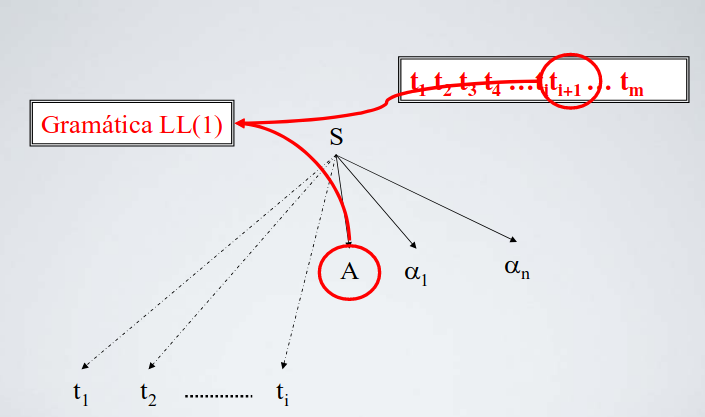
\includegraphics[width=0.5\linewidth]{img/33}
	\caption{Gramática LL(1)}
	\label{fig:4}
\end{figure}
\clearpage 

\section{Cálculo de Iniciales, Seguidores y Símbolos de predicción}
Para poder realizar el cálculo de los símbolos de predicción de nuestra gramática y poder generar nuestro \textbf{ASD} predictivo tendremos que definir la operación \textbf{Iniciales($\Upsilon$)}.
\subsection{Iniciales}
\textbf{Iniciales($\Upsilon$)} es el conjunto de símbolos terminales que pueden comenzar cualquier cadena generada por $\Upsilon$ ($\Upsilon$$\epsilon$(V$\cup$T)+)
\newline
\newline
¿Qué ocurre cuando la cadena vacía $\epsilon$ pertenece al conjunto Iniciales de alguna cadena?
\newline
Tenemos que seguir leyendo de la entrada y obtener el terminal de esa producción, o el terminal que derive del siguiente No-terminal. \cite{PL2}
\newline
\newline
\begin{figure}[h]
	\centering
	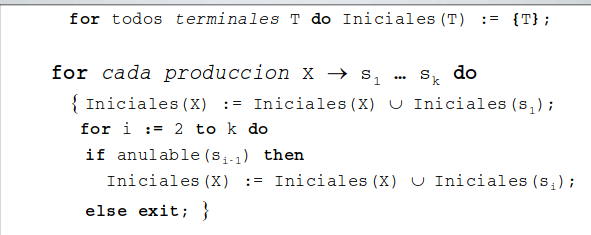
\includegraphics[width=0.7\linewidth]{img/ini}
	\caption{Cálculo iniciales}
	\label{fig:ini}
\end{figure}

Necesitamos entonces el concepto de \textbf{Anulables(X)}.
\subsubsection{Anulables}
\textbf{Anulables(X)} será igual a \textbf{True} si el No-terminal X puede generar $\epsilon$.
\begin{figure}[h]
	\centering
	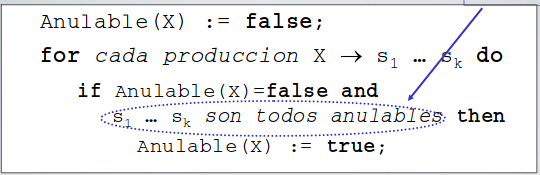
\includegraphics[width=0.7\linewidth]{img/an}
	\caption{Cálculo anulables}
	\label{fig:an}
\end{figure}
\clearpage
\subsection{Seguidores}
La operación \textbf{Seguidores(X)} calcula el conjunto de símbolos terminales t que pueden aparecer inmediatamente después del símbolo no terminal X, es decir hay una derivación desde el símbolo inicial, a una cadena con la forma $\alpha$\textbf{X}t$\beta$. \cite{PL2}

\begin{figure}[h]
	\centering
	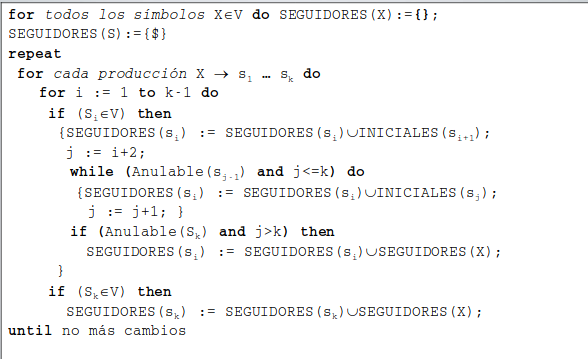
\includegraphics[width=0.7\linewidth]{img/seg}
	\caption{Calculo seguidores}
	\label{fig:seg}
\end{figure}

Esta operación que parece más compleja, realmente es sencilla, simplemente al calcular los seguidores de un No-terminal, tenemos que buscar ese No-terminal en las partes derechas de las producciones, y buscar los símbolos terminales que estén más a su derecha, y si estos fueran anulables (los No-terminales) tendríamos que calcular los iniciales del siguiente terminal o No-terminal.

\subsection{Símbolos de predicción}
Los símbolos de predicción es lo que realmente necesitamos para construir nuestro \textbf{ASD} predictivo pero para llegar hasta aquí necesitamos las operaciones anteriores.

\begin{figure}[h]
	\centering
	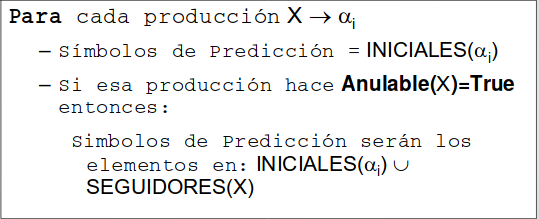
\includegraphics[width=0.7\linewidth]{img/predict}
	\caption{Cálculo de símbolos de predicción}
	\label{fig:seg}
\end{figure}

\clearpage
\section{Condición LL(1)}
\label{sec:ll1}
¿Qué propiedades ha de tener una gramática para que esta en particular sea LL(1)?
\begin{itemize}
	\item No puede ser recursiva a la izquierda
	\item Para cada producción X $\longrightarrow$ $\alpha_1$ | ... | $\alpha_k$ se tiene que cumplir que sus símbolos de predicción sean distintos, o lo que es lo mismo: \begin{itemize}
		\item  \textbf{Iniciales}($\alpha_i$) $\cap$ \textbf{Iniciales}($\alpha_j$) = $\emptyset$
		\item Si es \textbf{Anulable(X)} entonces:  \textbf{Iniciales}($\alpha_i$) $\cap$ \textbf{Seguidores}(X) = $\emptyset$
	\end{itemize}
	
\end{itemize}

\section{Gramática con recursividad por la izquierda}
\label{sec:hello}
Presentamos una gramática con el siguiente conflicto a resolver, es recursiva por la izquierda, para una mejor comprensión se utilizará la sintaxis \textbf{Proletool} \cite{Proletool} al indicar todas las gramáticas en el trabajo, pero antes ¿Qué es la recursividad por la izquierda?
\subsection{Recursividad por la izquierda}
Una gramática es \textbf{recursiva por la izquierda} cuando existe una derivación del tipo  $A \stackrel{*}{\Longrightarrow} A \alpha$
\newline
\newline
En particular, una gramática es recursiva por la izquierda si contiene una regla de producción de esa forma, en este caso la recursividad sería indirecta.
\newline
\newline
Ya sabemos que cuando la gramática es \textbf{recursiva por la izquierda} el análisis descendente predictivo no funciona, por ello tenemos que eliminarla.
\newline
\newline
\subsection{Gramática}
\begin{lstlisting}[caption = Gramática recursiva a la izquierda, style= Python]

grammar ejercicio_1{
analysis LL1;
nonterminal programa, metodo, cuerpo;
terminal class, end, def, ops, other_exp;

programa := class metodo end programa |;
metodo := metodo def | cuerpo ':';
cuerpo := ops | other_exp |;
}


\end{lstlisting}

\chapter{Análisis sintáctico ascendente}


\backmatter
% bibliography, glossary and index would go here.

\begin{thebibliography}{99}
	\bibitem{PL1} Apuntes de la asignatura de Procesadores de lenguajes, Tema 3 Análisis Sintáctico
	\bibitem{PL2} Apuntes de la asignatura de Procesadores de lenguajes, Tema 4 Análisis Sintáctico Descendente
	\bibitem{fact} Factorización de una gramática libre de contexto  y eliminación de recursividad por la izquierda, Universidad de Costa Rica, Escuela de ciencias de la computación e informática :\url{http://www.di-mare.com/adolfo/cursos/2009-2/pp-A73280-A73372-A76757.pdf}
	\bibitem{Proletool} Proletool, Software para la enseñanza y aprendizaje de Procesadores de Lenguajes
	
\end{thebibliography}
\end{document}